\documentclass[a4paper,11pt]{report}
% Preamble start

\usepackage{listings}
\usepackage{color}
\usepackage{graphicx}
\usepackage{rotating}
\usepackage{wallpaper}
\usepackage{hyperref}

\lstset{
	tabsize=4,
	language=sql,
	basicstyle=\scriptsize,
	%upquote=true,
	aboveskip={1.5\baselineskip},
	columns=fixed,
	showstringspaces=false,
	extendedchars=true,
	breaklines=true,
	prebreak = \raisebox{0ex}[0ex][0ex]{\ensuremath{\hookleftarrow}},
	frame=false,
	showtabs=false,
	showspaces=false,
	showstringspaces=false,
	captionpos=b,
	numbers=left,
	numberstyle=\tiny\color[rgb]{0.2,0.2,0.2},
	identifierstyle=\ttfamily,
	keywordstyle=\color[rgb]{0,0,1},
	commentstyle=\color[rgb]{0.133,0.545,0.133},
	stringstyle=\color[rgb]{0.627,0.126,0.941},
}

% Preamble end
\begin{document}
\ThisLRCornerWallPaper{1}{images/uabottomwave.pdf}
\ThisURCornerWallPaper{0.2}{images/logo_UA_U_kl3.pdf}
\ThisLLCornerWallPaper{0.3}{images/logo_UA_tekst_kl.pdf}
% Title page
\title{Inputlog Developer Documentation}
\author{}
\maketitle

% Table of Contents
\tableofcontents
\chapter{Algemene Info}
\section{Geschiedenis}
InputLog v5 is een complete rewrite van het oorspronkelijke Inputlog programma, in C\# 4.0 en Visual Studio 2010. De starterguide geeft uitleg ivm installatie en een kort overzicht van alle deelprojecten in de Inputlog solution. 

De huidige versie is ontwikkeld en uitgebreid door de volgende personen, in chronologische volgorde:
\begin{itemize}
\item Robbe Block \& Joris Roovers
\item Tom Pauwaert
\item Joeri Rammelaere
\item Robin Verschoren (PauseLocationMarker)
\item Matteo De Wint
\end{itemize}

\section{IDFX files}
De gelogde events uit inputlog sessies worden weggeschreven in een idfx bestand. Intern is een idfx een XML-bestand met root element \texttt{log}. Een log begint steeds met de elementen \texttt{meta} en \texttt{session}. Daarna volgen nul of meer \texttt{event}s die de acties weergeven die tijdens de sessie werden uitgevoerd.

\subsection{MetaInfo}
De MetaInfo bevat een unique identifier en de versie waarmee de logging werd uitgevoerd, maar belangrijker: timing informatie.
\begin{description}
\item[LogCreationDate:] String versie van de lokale DateTime op het moment van logging. Dit was oorspronkelijk de enige timestamp, wat problemen gaf met idfx bestanden die in een andere tijdszone werden gelogd etc. Wordt behouden voor backwards compatibility, ondertussen geniet de LogCreationTimeStamp de voorkeur.
\item[LogCreationTimeStamp:] UNIX timestamp in milliseconden van de universele tijd op het moment van logging. Indien aanwezig zal deze binnen het programma (de getters in klasse \texttt{SessionIdentification}) de LogCreationDate overriden.
\item[LogRelativeCreationDate:] Aantal milliseconden tussen het moment waarop de computer werd opgestart en het begin van de logging. Alle tijden van events worden ook opgeslagen als het aantal milliseconden verstreken sinds het booten, dus door hier de LogRelativeCreationDate van af te trekken kan je de starttijd van het event bekomen, relatief ten opzichte van het begin van de logging. In de programmacode wordt dit tegenwoordig de RelativeCreationTime genoemd omdat het weinig met dates te maken heeft, maar vanwege compatibility kan dit niet in de idfx veranderd worden.
\end{description}

\subsection{SessionInfo}
Dit element bevat de waarden die werden ingevuld in het ``Session identification'' venster op de Record tab van Inputlog: Participant, Text Language, Age, \ldots

\subsection{Events}
Ieder event heeft een ID en een type, meestal Mouse, Keyboard of Focus. In een normaal idfx bestand bevindt zich helemaal op het eind ook een Statistics event. Een overzicht van alle mogelijke event types kan je vinden in klasse  InputLog.Core.Events.EventType. 

Binnen een event kunnen verschillende EventParts voorkomen. Bij een normale logging zal een Keyboard event bijvoorbeeld een winlog en wordlog part hebben, met gegevens die respectievelijk via een windows en een word hook werden bekomen. Zoals eerder vermeld worden StartTime en EndTime uitgedrukt in milliseconden sinds het booten.

\chapter{Analyses}
\section{Adding a new analysis}
Note: Inputlog uses reflection in some classes in order to minimize the amount of work that is needed to add a new analysis. By doing so, we rely on some naming conventions of the classes implementing analyses. Specifics about this in the steps below.

In order to add a new analysis, you should perform the following steps:
\begin{enumerate}
\item Create the Analysis itself in InputLog.Core project/Analyses. The easiest way to do this is by copying an existing Analysis (e.g. GeneralAnalysis). Make sure to also copy the Summary and XML writer/serializer classes from this analysis.
\item Update the copied Analysis class and file names (do not forget to update the namespace!). It's probably a good idea not to include any new functionality just yet, but do that after you have succesfully added the new analysis (so that you can run it from the GUI). Note that you should follow the naming conventions of the names of the classes (that is, use ``MyNewAnalysisXMLWriter'' for the XMLWriter; do the same for the other classes) as some reflection is used to instantiate these classes later on.
\item Create a new XSL stylesheet for the new analysis in InputLog.Core project/Analyses/Styles. Again, it is probably the easiest to copy an existing style and rename the file.
IMPORTANT: In order to include the new stylesheet in the release, you have to change the default property ``Copy to Output Directory'' value from ``Do not copy'' to ``Copy if newer''. This can only be done while running Visual Studio with Administrator rights.
\item The Analysis itself is now created; we now need to add it to the GUI.
\item Copy an existing AnalysisControl folder under the GUI/Tabs/Analyze/AnalysesControls, for example the Bigram/ folder.
\item Update the file names and the class names of the copied control (both analyzer and analysiscontrol). Remember to both change the names and classnames in MyNewAnalysis.cs and MyNewAnalysis.designer.cs
\item Update the GUI of this new analysis control (in particular, you might want to change the name label, leave more complex changes for later...).
\item Update the copied classes
\begin{enumerate}
\item MyNewAnalysisControl.cs: Update ProduceAnalyzer() method to create a new MyNewAnalyzer()
\item MyNewAnalyzer.cs: Change the NAME and ABBR constants
\item MyNewAnalyzer.cs: Update the GetAnalysis() method to return the new analysis
\item MyNewAnalyzer.cs: Update GetParameters() method to store analysis config
\item Update comments!
\end{enumerate}
\item Add MyNewAnalysis to the 'Analyses' dictionary (private field) in GUI Project/Tabs/Analyze/Analyze.cs. No further changes to Analyze.cs are needed (all necessary changes are taken into account using reflection).
\item That should be it :-)
\end{enumerate}

\section{AbstractAnalyzer flow}
\begin{enumerate}
\item StartSession
\item SetPaths
\item PreProcess
\item DoAnalysis
\item WriteAnalysis
\end{enumerate}

\section{Analyzer Hooks}
De klasse AbstractAnalyzer stelt verder nog een aantal virtuele functies ter beschikking voor afgeleide analyses:
\begin{description}
\item[string ExtendFileName:] Bepaalt de bestandsnaam van de uitgeschreven analyse, overriding is nuttig om extra parameters in de bestandsnaam op te nemen
\item[bool BeforeAnalysis:] Wordt uitgevoerd voor de analyse, als false wordt gereturned wordt de analyse geannuleerd
\item[void AfterAnalysis:] Wordt uitgevoerd na de analyse, krijgt summary als parameter
\item[bool BeforeWrite:] Wordt uitgevoerd voor het uitschrijven van de analyse, indien true wordt gereturned
\item[void AfterWrite:] Wordt uitgevoerd na het uitschrijven van de analyse
\end{description}

\section{Process Graph Analysis}
De Process Graph Analysis geeft een grafische voorstelling van een General Analysis. Het proces werkt door eerst een General Analysis uit te voeren en weg te schrijven, en deze vervolgens te laten inlezen door een VisualizationForm (zie namespace Visualization). Het eigenlijke inlezen gebeurt in klasse VisualizationDataPoint, waarlangs een lijst van VisualizationDataPoints bekomen kan worden. Deze points bevatten de info die uiteindelijk geplot wordt.
\subsection{Series togglen}
De verschillende chart series kunnen getoggled worden door de linklabels in de legende. Na iedere toggle worden alle series opnieuw getekend. De toggle zelf flipt een boolean die aangeeft of de serie in kwestie getekend moet worden. Bij het opnieuw tekenen worden alle series verwijderd, en vervolgens wordt per serie een functie aangeroepen. Deze functie gaat na of de serie getekend moet worden, voegt de datapunten toe indien nodig, en voegt anders een ``dummy-serie'' toe met dezelfde settings (om de legende intact te houden).
\subsection{Focus serie}
Net boven de x-as wordt een lijn getekend indien het gelogde document de focus heeft. Om te bepalen welk document dit is en of het de focus heeft, wordt gekeken naar de focuschange events in de analyse. Er wordt verondersteld dat het eerste Word-document waarnaar geswitcht wordt, het main document is.
Om de focuslijn te tekenen wordt gebruik gemaakt van het aantal pixels per interval op de grafiek (momenteel 65). Dit om te vermijden dat de focuslijn door de x-as gaat ipv er bovenop te liggen. Wanneer de intervals of de grootte van de grafiek aangepast worden, moet dit dus ook aangepast worden.
\subsection{Interactieve view openen}
Bij het uitvoeren van een process graph analyse wordt de ``open file'' link in de AnalysisControl misbruikt om de interactieve view te openen. Het VisualizationForm wordt op voorhand klaargemaakt en enkel getoond wanneer hierop geklikt wordt. Daarnaast wordt het niet echt gesloten wanneer men op de sluitknop klikt, enkel verborgen (anders zou de volledige analyse iedere keer opnieuw ingelezen moeten worden wanneer het venster geopend wordt). Dit venster wordt definitief gesloten en verwijderd wanneer de AnalysisControl verwijderd wordt uit de lijst.

\section{Fluency Analysis}
\subsection{Algemene flow}
De Fluency Analysis volgt het proces van een gewone analyse. De parameters zijn grotendeels hetzelfde als voor de Linear Analysis, die als basis dient voor de fluency. Na het uitvoeren van de Linear wordt in de Fluency Analysis over alle periodes uit de linear gelopen, om per periode de fluency statistieken te berekenen. De minimale grote voor een interval om in de fluency analyse beschreven te worden, wordt bepaald door de constante PERIOD\_MIN\_SIZE in de Core FluencyAnalysis, standaard 10 seconden. Deze ondergrens is nodig om in het geval van focus of revisie intervals nietszeggende pieken en dalen te vermijden.
\subsection{Optima}
\begin{description}
\item[Absolute:] Dit optimum wordt bepaald door de constante \hfill\\DEFAULT\_ABSOLUTE\_OPTIMUM in de Core FluencyAnalysis. Er zijn voorziening om deze eventueel in het register weg te schrijven via het opties-menu (en vervolgens in te lezen), maar dit is momenteel uitgeschakeld
\item[Personal:] Het personal optimum wordt ingegeven via de FluencyAnalysisControl in de GUI. Het veld in de GUI wordt steeds ingevuld met de waarde die is opgeslagen in het register. Het personal optimum kan opgeslagen worden via het opties-menu, of via de FluencyAnalysisControl. Voor dit laatste verschijnt een save-link van zodra de waarde wordt aangepast, en ook het task optimum van een taak kan opgeslagen worden om in de toekomst als personal optimum te dienen
\item[Task:] Het task optimum wordt berekend als de maximale waarde van een voortschrijdend gemiddeld. Dit gemiddelde wordt genomen over de (minimale) lengte van \'e\'en interval. Als deze minimale lengte gelijk is aan $l$, wordt een tweede linear analysis uitgevoerd met intervals van lengte $\frac{l}{w}$, waarbij $w$ via een inverse faculteit beperkt groeit naarmate $l$ groter wordt, zie tabel hieronder. Over deze intervals wordt een voorschrijdend gemiddelde berekend met window $w$. Het maximale voortschrijdende gemiddelde wordt beschouwd als Task Optimum.\\
\begin{tabular}{c|c}
$l \geq 10s$ &$w = 2$\\
$l \geq 1m$ &$w = 3$\\
$l \geq 3m$ &$w = 4$\\
$l \geq 12m$ &$w = 5$\\
$l \geq 1h$ &$w = 6$\\
\end{tabular}
\end{description}

\subsection{Grafische weergave}
Voor de grafische weergave wordt de klasse FluencyGraph gebruikt. Er zijn 2 varianten: een FluencyGraph voor \'e\'en enkele analyse, en een MultiFluencyGraph om meerdere analyses te vergelijken. Het enige verschil is dat in de enkelvoudige FluencyGraph de waarden voor alle analyses tegelijk worden geplot, terwijl de MultiFluencyGraph slechts \'e\'en optimum tegelijk toont voor de verschillende analyses. Voor een gegeven optimum wordt zowel een lineplot als een trendlijn getoond, waarbij de trendlijn een spline is die door beginpunt, eindpunt en gemiddelde van de 2 of 3 middenste punten van de lineplot. Per analyse wordt ook de zone getoond waarin het task optimum behaald werd, in de vorm van een column plot.

In de FluencyAnalysisControl wordt per analyse een enkelvoudige FluencyGraph opgemaakt, die wordt uitgeschreven naar een afbeelding. Indien er meerdere idfx files worden opgegeven (tegelijkertijd of \'e\'en per \'e\'en zonder intervals te wijzigen), wordt bij de 2de analyse een MultiFluencyGraph gegenereerd die de eerste 2 analyses bevat. Verdere analyses worden hieraan toegevoegd. De grafiek wordt getoond via de ``Show Graph'' link die in de GUI getoond wordt na afloop van de analyse. In deze grafiek kunnen alle plots getoond of verborgen worden.

\chapter{WebApp en Server}
\section{Client-Server architectuur}
De client-server architectuur is ingevoerd vanwege een specifieke nood: linguistische analyses zijn niet (sc)haalbaar voor een lokale installatie.
De effectieve implementatie is echter zodanig dat alle analyses potentieel op de server uitgevoerd kunnen worden.

De werking is als volgt: de gebruiker selecteert de analyses op de normale manier. Indien het een server-analyse betreft, zal de gebruiker een popup krijgen om in te loggen. Hierna wordt een beschrijving van de analyse naar de server verzonden. Deze server zal de analyse na verloop van tijd uitvoeren. Als de analyse uitgevoerd is, zal de gebruiker eventueel via email op de hoogte gebracht worden. Wanneer hij heeft besloten te wachten op de resultaten, en de Inputlog client nog draait, zal het resultaat meteen gedownload worden, en net zoals bij andere analysis in de Inputlog map geplaatst worden. Daarnaast zal de gebruiker via een webinterface in staat zijn om de resultaten op te vragen.

Om praktische redenen is de server onderverdeeld in een console applicatie die de analyses uitvoert en een webapplicatie die de administratie regelt.

\section{Server-analyse toevoegen}
De analyse op zich (in InputLog.Core.Analyses) kan gecodeerd worden als ware het een lokale analyse. Het enige verschil is dat er een serializable AnalysisDescription voor de analyse aangemaakt moet worden (zie InputLog.Core.Analyses.General.GeneralAnalysisDescription voor een voorbeeld).

De AnalysisControl in de Client GUI dient over te erven van de klasse ServerAnalysisControl. De flow van deze control werkt als volgt:
\begin{enumerate}
\item In de constructor maakt de ServerAnalysisControl een tijdelijke map aan, waarvan het pad terug te vinden is in attribuut TempDir. Hierin komen de geserializeerde AnalysisDescriptions terecht. Deze TempDir heeft een subdirectory Work waarin extra benodigde bestanden geplaatst kunnen worden door AnalysisControls (bijvoorbeeld om het originele word document mee te sturen). De methode Analyze() kan overridden worden om per idfx bijvoorbeeld een document in de Work directory te plaatsen.
\item Per idfx file wordt de methode Analyze() aangeroepen. Deze methode zal eerst de gebruiker laten inloggen op de server. Daarna wordt de methode PreProcess() uit IAnalysisControl aangeroepen. Vervolgens wordt binnen Analyze() de polymorfe methode GetAnalysisDescription() opgeroepen. Deze AnalysisDescription wordt geserializeerd en gegzipt weggeschreven naar TempDir.
\item Wanneer alle idfx files gepasseerd zijn door de Analyze() methode, zal ServerAnalysisControl.Launch() aangeroepen worden (enkel voor AnalysisControls die overerven van ServerAnalysisControl!). Deze methode zal de bestanden in TempDir zippen en versturen naar de WebApp. Vervolgens wordt een timer gestart, die elke minuut nagaat of de analyse al gefinisht is.
\item Als de analyse afgewerkt is op de server, in methode ProbeTimer\_Tick() de summaries gedownload via de WebApp en uitgeschreven naar de lokale InputLog directory.
\item GUI-matig wordt verondersteld dat iedere ServerAnalysisControl een ProgressBar en een StatusLabel ter beschikking stelt. De methodes GetProgressBar() en GetStatusLabel() dienen overridden te worden om referenties naar deze twee controls terug te geven.
\end{enumerate} 

\section{Server: Analyses}
\subsection{Algemene werking}
De Serverapplicatie bevat een TaskManager, die een bepaald aantal TasksExecutors zal lanceren in aparte threads. De TaskManager scant de database, haalt Tasks op uit de wachtrij, start een TaskExecutor per Task, en markeert de Task als Pending wanneer ze gestart wordt en als Completed wanneer ze afgelopen is.
\subsection{Input structuur}
Iedere gebruiker heeft een subfolder in de workdirectory, en iedere Task van deze gebruiker krijgt een aparte folder binnen deze gebruikersfolder.
Hierin wordt de Input-zip geplaatst die de WebApp heeft ontvangen.
De inhoud van deze zip ziet er als volgt uit:
\begin{itemize}
\item[-] Work (map met bestanden voor specifieke analyses, zoals original Word documents)
\item[-] input.xml.gzx (analysis description voor iedere idfx file, gzipped; x volgorde van het bestand - nodig voor meerdere idfx bestanden)
\end{itemize}
\subsection{Output structuur}
Output bestaat uit 2 delen: enerzijds wordt er een bestand Results.zip gemaakt met alle outputbestanden (output-x.xml), en de nodige stylesheets en dergelijke. Anderzijds wordt er ook een bestand Summaries.zip gemaakt van de verschillende summaries, die door de client wordt opgevraagd waarna de resultaten lokaal worden uitgeschreven. Deze zip bevat bestanden Summary.xml.gzx (serialized summary, gzipped; x volgorde van het bestand - nodig voor meerdere idfx bestanden)
	
\section{WebApp: Administratie}
\subsection{Technische details}
	\begin{itemize}
		\item ASP.NET MVC3
		\item RazorEngine
		\item MySQL
	\end{itemize}
\subsection{Registratie en login}
Registratie en login worden afgehandeld door de AccountController.
Gebruikers registreren met gebruikersnaam, email en wachtwoord. Minimale wachtwoordlengte is gedefinieerd in de algemene web.config, in de settings voor de Membership Provider. Wachtwoorden kunnen aangepast worden, of gereset (auto-generated wachtwoord wordt gemaild naar de gebruiker). Tenslotte is er e-mailvalidatie nodig vooraleer gebruikers hun account kunnen gebruiken.
\subsection{Roles}
Standaard zijn er drie rollen voorzien in de database: Disabled, Default en Admin. Gebruikers die hun e-mailadres gevalideerd hebben, komen in Default terecht. Na verwijdering van hun account (zelf of door Admin) komen ze in Disabled terecht. Disabled accounts kunnen niet inloggen en dus ook geen acties uitvoeren, maar zitten nog in de database voor de eventuele statistieken. Admins kunnen analyse-types toevoegen en andere gebruikers verwijderen of admin maken.
Zie AccountController.Validate() voor een voorbeeld om gebruikers aan een Role toe te voegen/uit een Role te verwijderen.
\subsection{Shared views}
\begin{description}
	\item [Error:] View die gebruikt wordt voor alle errorpagina's
	\item [Master:] Standaard paginalayout die op alle views wordt toegepast
	\item [Value:] View die gebruikt wordt om een enkele waarde terug te geven (aan de client applicatie). Zou in de toekomst beter via zuivere XML api gebeuren
\end{description}
\subsection{Emails}
Het emailsysteem werkt met behulp van de library Postal:\\
\href{http://aboutcode.net/postal/}{http://aboutcode.net/postal/}
De inhoud en layout van emails werkt net zoals gewone views. Layout wordt momenteel niet gedeeld tussen de emails. Voorbeelden zijn te vinden in de map Views/Emails
\subsection{Configuratie}
Het algemene web.config bestand bevat de volgende aangepaste elementen:
\begin{itemize}
	\item Connectiestring voor MySQL database (connectionStrings)
	\item URL van het login formulier (authentication)
	\item Custom profielvelden (profile/properties)
	\item SMTP server instellingen (mailSettings)
	\item Site URL en Server applicatie directory (appSettings)
\end{itemize}
\subsection{Interactie met server}
De WebApp ontvangt Tasks en slaat deze op in de database. De inputbestanden worden door de WebApp in de workdirectory van de server geplaatst. De WebApp haalt in deze directory de resultaten op wanneer deze gevraagd worden. Wanneer TaskController.SendNotifications() wordt aangeroepen, zal de WebApp mails versturen voor Tasks die wel afgewerkt zijn, maar nog niet gedownload.
\subsection{Database}
	De WebApp database bevat slechts drie Inputlog-specifieke tabellen: voor de entiteiten Task en Analysis en hun relaties. De andere benodigde tabellen zijn automatisch gegenereerd voor de ASP Membership en Profile providers.\\	\href{http://msdn.microsoft.com/en-us/library/yh26yfzy(v=vs.100).aspx}{http://msdn.microsoft.com/en-us/library/yh26yfzy(v=vs.100).aspx}
	\begin{description}
		\item [Task:] Een enkele analysis request verstuurd door de client. Een Task kan meerdere idfx files omvatten.
		\item [Analysis:] Naam van een analyse die uitgevoerd kan worden op de server. Dit heeft vooral statistisch nut, zolang er niet rechtstreeks analyses ``besteld'' worden via de WebApp. Welke analyse effectief uitgevoerd wordt, hangt enkel af van de Description die door de client wordt verzonden. Een Task kan aan meerdere Analyses gekoppeld worden (for the sake of flexibility).
	\end{description}
	\begin{figure}
		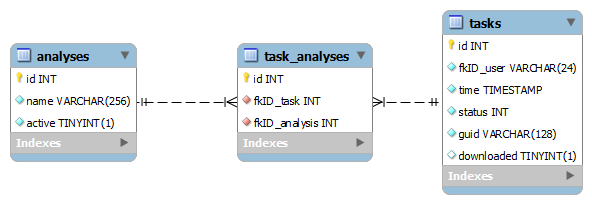
\includegraphics[width=5.5in]{images/ileer.png}
		\caption{ER diagram server}
	\end{figure}
	
\section{Server machine}
\subsection{Details}
\begin{itemize}
\item Hostname: Inputlog.ua.ac.be
\item Ip adres: 143.169.247.36
\item Windows server 2008R2
\item Remote desktop vanaf 146.175.120.186 (Z.503) en  146.175.120.177 (Z.504)
\item Tivoli backup client (backup van de database moet apart op disk gemaakt worden)
\item IIS webserver
\item Nsclient++ monitoring agent
\item Antivirus
\item Vmwaretools
\item MySQL 5.5.27
\item MySQL NET Connector 6.5.4 \& ODBC Connector 5.1.11
\item .NET Framework 4
\end{itemize}

\subsection{Accounts}
\subsubsection{Admin account}
\begin{itemize}
\item login: luuk
\item Paswoord: XXXXXX (same as calliope)
\end{itemize}

\subsubsection{MySQL root account}
\begin{itemize}
\item login: root
\item Paswoord: XXXXXX (same as calliope)
\end{itemize}

\subsubsection{MySQL WebApp account}
\begin{itemize}
\item login: inputlog
\item Paswoord: PeperEnZout
\end{itemize}

\subsection{Directories}
\begin{description}
\item[WebApp:] C:\textbackslash inetpub\textbackslash  wwwroot\textbackslash  WebSite
\item[ServerApp:] C:\textbackslash  Inputlog\textbackslash  ServerApp
\end{description}
	
\chapter{Inputlog Lite}
Inputlog Lite is een speciale versie van Inputlog, waarin niet de analyses centraal staan maar wel de logging. Deze versie is voornamelijk bedoeld om door schrijvers te worden gebruikt, niet door wetenschappers. Behalve de logging bevat Inputlog lite ook functionaliteit om schrijfprojecten te beheren en te organiseren. De IDFX bestanden van de logging worden geupload naar de WebApp.

\section{Programma Flow}
Bij het opstarten wordt er gekeken of er in de registry een Workspace directory is opgeslagen, zoniet wordt het startup formulier getoond. De projecten worden ingelezen uit de workspace directory, als er nog geen projecten zijn wordt het new project formulier getoond. Het meest recent aangepaste project wordt als huidig project ingeladen, waarna een dialoogvenster wordt getoond met de vraag of de gebruiker wil verdergaan met dit project.

Indien niet wordt de main GUI getoond, met links de gegevens van het huidige project en rechts de knoppen:
\begin{description}
\item[Blank Document:] Voegt een nieuw document toe aan het huidige project
\item[Existing Document:] Opent een bestaand document, indien dit in een project zit wordt dit project geladen, zoniet wordt het document gekopieerd naar het huidige project
\item[Experimental Flow:] Opent een zip met een opeenvolging van templates voor een logsessie, hiervoor wordt een nieuw project aangemaakt
\item[Record:] Start een record sessie
\end{description}
Een nieuw project kan worden aangemaakt door ``new'' te selecteren in het dropdown menu, dit wordt intern weergegeven door de klasse NewProjectEntry.

Tijdens het loggen worden alle buttons gedisabled. Na het loggen wordt het idfx bestand geupload naar de inputlog server, indien mogelijk. Anders wordt het idfx bestand toegevoegd aan de lijst DelayedIdfxs van het betreffende project. Bij het opstarten van het programma wordt telkens geprobeerd de DelayedIdfxs te verzenden naar de server.

\section{Workspace structuur}
Binnen de geselecteerde workspace wordt een folder ``Projects'' aangemaakt voor de Lite versie. Binnen Lite worden sessies georganiseerd binnen projecten: een project bevat \'e\'en of meerdere documenten met eenzelfde auteur en taal, en in principe eenzelfde thema/onderwerp/\ldots. Ieder project heeft een eigen map in de workspace, en binnen het project heeft ieder document een eigen map: hierin worden het document, de idfx bestanden, en de backups van het document voor iedere logging sessie opgeslagen. De volgende afbeelding geeft een voorbeeld van de structuur:
	\begin{figure}[H]
		\centering
		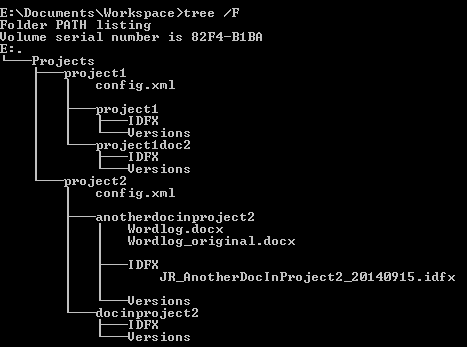
\includegraphics[width=3.5in]{images/litefolder.png}
		\caption{Lite folder structuur}
	\end{figure}
	
\section{Xaml}
Hier een korte beschrijving van de verschillende Xaml files in het project
\begin{description}
\item[AddDocument:] Textbox om de naam van een nieuw document in te geven
\item[FolderEntry:] Kies-workspace dialoogvenster
\item[LastWords:] Textbox waarin je een opmerking kunt opgeven na het loggen
\item[MainWindow:] Hoofdvenster
\item[NewProject:] Venster voor het aanmaken van een nieuw project
\item[ProjectOverview:] Niet meer gebruikt, bevatte een lijst van projecten
\item[ProjectProperties:] Niet meer gebruikt, diende om properties van projecten aan te passen
\item[StartupForm:] Formulier dat bij eerste opstarten wordt getoond (en via File: Settings), om workspace en account in te vullen
\item[Styles:] Bevat enkele herbruikbare templates
\end{description}

\chapter{Various}
\section{EmbeddedWord}
Alvorens je dit project kan compileren, moet je erop letten dat in de project properties het paswoord van het ondertekenen is ingesteld (zoals dat ook met het core project moet: Properties => Signing => key file = EmbeddedWordKey.pfx, pwd = PeperEnZout). Ook de referenties moeten correct staan (in het bijzonder moet de referentie DSOFramer waarschijnlijk bij jullie opnieuw toegevoegd worden, dit is 'DSOFramer.dll' in de submap Resources. Het GUI project leunt nu op zowel het Core project als op het Embedded Word project (maar ik denk dat deze settings wel via svn correct worden overgenomen) en ook de DSOFramer refentie dient in dit project to worden toegevoegd.

\section{Pause Location Marker}

	The PauseLocationMarker was reimplemented using a more explicit finite state machine.
	It is now possible to specify the recognized rules (i.e. sequence of specific Events) and actions to take upon recognizing these rules in the form of regular expressions.
	These rules are represented in the text file ``InputLog/Core/Analyses/PauseParser/FSMRules.txt'', which should be copied when building the project.
	
	
	The possible triggers used in these rules should be implemented in a class that implements the IEventLookup interface, which can then be used in the PauseLocationMarker itself.
	The possible actions used in these rules should be implemented in a class that implements the IActionLookup interface.
	\subsection{Rule syntax}
		\newcommand{\syntsubst}[1]{<#1>}	%Rule substitution
		\newcommand{\syntlit}[1]{'#1'}		%Literal
		\newcommand{\syntrept}[1]{#1*}		%Optional arbitrary repetition
		\newcommand{\syntopt}[1]{\syntparen{#1}?}		%Optional 0 or 1 repetition
		\newcommand{\syntparen}[1]{(#1)} 	%Parentheses
		\newcommand{\syntclass}[1]{[#1]}	%Character class	
		The text file uses a simple regular expression-like syntax. In the following description of the syntax, the following list of conventions is assumed:
		\begin{description}
			\item[$\syntsubst{syntrule}$]:\\describes a substitution of another syntax rule; 
			\item[$\syntlit{literal}$]:\\describes a literal string; 
			\item[$\syntopt{opt}$]:\\describes an optional part and thus, this  can be left out;
			\item[$\syntrept{rept}$]:\\describes a part that can be repeated an arbitrary number of times (includes 0 repetitions);
			\item[$\syntparen{paren}$]:\\groups different rules together;
			\item[$\syntclass{class}$]:\\describes a character class. Reading any character of the class results in accepting the rule.
		\end{description}
		
		Please note that all whitespace characters are ignored and should be removed by the generated scanner.
		\subsection{Rule syntax description}\label{pauselocmarkerrulesyntax}
		\begin{description}
			\item[Identifier]:\\
				$\syntclass{A-Za-z}\syntrept{\syntclass{A-Za-z0-9}}$\\
				An identifier corresponding to an event or action that can be looked up by the IEventLookup and IActionLookup classes. It begins with a letter, followed by an arbitrary number of letters and digits.
			\item[Trigger]:\\
				$\syntopt{\syntlit{!}} \syntsubst{identifier} \syntopt{\syntparen{\syntlit{<} \syntopt{\syntlit{-}}\syntclass{0-9}}\syntrept{\syntclass{0-9}} \syntlit{>}}$\\
				This is one element in an list of trigger events. When $\syntlit{!}$ is present, it denotes the negation of the trigger event's outcome. When the latter part is present, it means that we will peek forward or backward (if the number is negative) in the currently inspected list of Events and execute the specified trigger event function on that Event in the list.
			
			\item[Trigger list]:\\
				$\syntsubst{trigger}\syntrept{\syntparen{\syntlit{,}\syntsubst{trigger}}}$\\
				This is a list of event identifiers.
			\item[Action list]:\\
				$\syntopt{\syntlit{\{} \syntsubst{identifier}\syntrept{\syntparen{\syntlit{,}\syntsubst{identifier}}}  \syntlit{\}}}$\\
				This is an optional list of action identifiers, surrounded by braces.	
			\item[Rule]:\\ 
				$\syntclass{\syntsubst{symbol} \syntsubst{parentheses} \syntsubst{kleenestar} \syntsubst{number} \syntsubst{plus} \syntsubst{union} \syntsubst{concatenation}} \syntsubst{actionlist}$\\
				This denotes one of the possible rules. The actions will be executed when the rule is recognized.
			\item[Symbol]:\\ 
				$\syntsubst{triggerlist}$\\
				This serves as the basic building block of the syntax and aims to recognize only one set of events at a time.
			\item[Parentheses]:\\ $\syntlit{\left(} \syntsubst{rule} \syntlit{\right)}$\\
				This serves as the basic building block of the syntax and aims to recognize only one set of events at a time.
			\item[Kleene Star]:\\ 
				$\syntsubst{rule} \syntlit{*}$\\
				This denotes an arbitrary number of repetitions of the subrule (0 or more times).
			\item[Plus]:\\ 
				$\syntsubst{rule} \syntlit{+}$\\
				This denotes one mandatory time that the subrule has to be recognized, followed by an arbitrary number of repetitions of the subrule (1 or more times).
			\item[Number]:\\
				$\syntsubst{rule} \syntlit{[} \syntclass{0-9}\syntrept{\syntclass{0-9}} \syntlit{]} $\\
				This denotes that the subrule has to be recognized the specified number of times.
			\item[Union]:\\ 
				$ \syntsubst{rule} \syntlit{|} \syntsubst{rule} $\\
				This denotes the union of 2 subrules. If at least one of them is true, the rule is accepted. It is a short-circuit operator (\url{https://en.wikipedia.org/wiki/Short-circuit_evaluation}). 
			\item[Concatenation]:\\ $ \syntsubst{rule} \syntlit{.} \syntsubst{rule} $\\	
				This denotes the concatenation (sequencing) of 2 subrules.		
			\item[Start]:\\ $ \syntsubst{rule}\syntlit{;} \syntrept{\syntparen{\syntsubst{rule}\syntlit{;}}}$\\	
				This is the start symbol of the syntax. Evaluation of input text begins here.
		\end{description}	
	 
	\subsection{Adding a new rule}
		\subsubsection{To the rule syntax}\label{pauselocmarkeraddruletosyntax}
			Adding a new rule to the syntax can be done quite easily.
		
			First determine a new symbol to be used and add this to the list of tokens in the Scanner.lex and Parser.y files in the Core.Analyses.PauseParser namespace. Also add a rule that recognizes the determined syntax to the grammar contained in the Parser.y file, for example in the productions of the compoundRule grammar symbol.
		
			In the semantic actions (the part between braces) of the newly added grammar rule in Parser.y, you can specify which actions to take when the new rule is recognized from the input file.
			This can include calls to an implementation class of the IRuleFactory interface.
		
			The best approach for these semantic actions is to create a new subclass of the abstract ARegexRule in the Core.Analyses.PauseParser.RegexRule.cs file with a descriptive name. The AddToFSM member method should be implemented with the semantics of the new rule and should make calls to the AFSMFactory argument. This factory contains methods for the most basic building blocks of epsilon non-deterministic finite state automata (\url{https://en.wikipedia.org/wiki/Nondeterministic_finite_automaton_with_\%CE\%B5-moves}). These building blocks can be linked together by making concatenations and unions, for which there are also methods in the AFSMFactory. The return values of each building block specify the start and end state identifiers in the finite state machine, which could and should be used as arguments for the methods to link the blocks.
		
			It should not be necessary to modify the AFSMFactory itself. However, to call the new rule from the Parser.y file, a public method needs to be added to the IRuleFactory interface and implementing classes, which constructs the new ARegexRule subclass. The new method of the IRuleFactory implementation can then be called in the semantic actions of the new grammar rule in the Parser.y file.
			
			Also, the syntax and semantics of the new rule should be added to \autoref{pauselocmarkerrulesyntax}.
			
		\subsubsection{To the rule input file}
			To add a new rule to recognize Events and determine the right PauseLocation for the Event in a list of Events, simply add a new line containing the necessary sequence of Events and actions to take upon recognition of that sequence to the FSMRules.txt file or another input text file that serves as an argument in the constructor of the PauseLocationMarker class.
			
			The syntax and semantics for these rules are described in \autoref{pauselocmarkerrulesyntax}.
			
			Priority for the rules in this file is higher when it appears earlier on in the file.
		
		
	\subsection{Revising rule implementations}
		\subsubsection{For the rule syntax}
			Revising the syntax rules can be done quickly by modifying the Scanner.lex and Parser.y files as seen fit. Documentation for the syntax required by the GPLEX and GPPG scanner and parser generators are available at \url{https://gplex.codeplex.com/} and \url{https://gppg.codeplex.com/}.
			
			For implementation guidelines of new features, we refer to \autoref{pauselocmarkeraddruletosyntax}.
			
		\subsubsection{For the input file}
			Determine the part of the Event sequence or semantic actions that should be modified in a specific rule in the FSMRules.txt text file (or another text file that is used in PauseLocationMarker to construct the finite state machines).
			
			Modify the trigger event sequences and/or actions in the line that needs to be modified in the FSMRules.txt file. The rule modifications should be enforced the next time the PauseLocationMarker code is run from the InputLog GUI or in the unit tests.
			
			No rebuilding should be necessary, except maybe to copy the revised text file to the build or binary directory, which can also be done manually. The text files can also be directly revised from the build or binary directory itself. These should also be located in the Analyses/PauseParser subfolder.
			
	\subsection{Implementing new trigger events or actions}
	
		Adding new trigger events or actions for use in the rule input text file for the PauseLocationMarker can be done quite easily.
		
		First, determine whether a new event or action is required and at which point in time it needs to be called. Insert the name of the event or action in the rule input text file, at the necessary location.
		
		
		Second, add the implementation to the IEventLookup or IActionLookup implementing classes, depending on the added functionality. The PauseLocationEvent- and PauseLocationActionLookup classes are used by default, so the new trigger event or action should be added in those classes.
		These classes use reflection to map a name or identifier unto a predicate (boolean returning function without arguments) or action (void returning function without arguments). This is done in the FindPredicate or FindAction methods of the lookup classes.
		
		The implementation of the new trigger event or action should be called the same as the name used in the input file, determined in the first step of these instructions. It should also be a \textbf{public} and \textbf{static} member method of the class and should have no formal parameters.
		If a specific name used in the input should be mapped to a different method (e.g. to a method requiring a parameter or a method with formal parameters), this mapping should be added to or modified in the FindAction or FindPredicate methods of the classes.

		

\section{Code Documentation}
	Documentation can now be extracted from source files by using \href{http://www.doxygen.org}{Doxygen}, by using the added Doxyfile (located in the root folder of InputLog).
	
	Step-by-step instructions:
	\begin{enumerate}
		\item Download and install Doxygen from \url{http://www.doxygen.org} if necessary.
		\item Open the Doxywizard application.
		\item Open the configuration file called Doxyfile from the "File$\rightarrow$Open..." menu. This file is located in the root folder of InputLog.
		\item Tweak the parameters in the Wizard and Expert tabs of the Doxywizard if necessary. For example, when new source folders are created, the input folders can be tweaked in the Expert tab, in the Input topic.
		\item Run Doxygen by clicking the "Run Doxygen" button in the Run tab of the Doxywizard. The output of Doxygen should appear in the windowpane in the wizard. This output could include helpful information, e.g. statements indicating undocumented parameters, methods and/or classes.
		\item By clicking on the "Show HTML Output" button, the HTML output of Doxygen is opened in the default HTML viewer. The main HTML file, which is called "index.html", is located in "Doc/Doxygen/html" when it is generated.
		
		Other output options, e.g. \LaTeX{} output, can be toggled in the Wizard tab, topic Output in the Doxywizard.
	\end{enumerate}
	

\section{Unit Tests}
	Unit testing was introduced. The tests use the open source \href{http://www.nunit.org/}{NUnit} testing framework and should be familiar to people with experience in xUnit based unit testing tools.
	The system was first tested under NUnit version 2.6.2.
	
	NUnit can be installed on a system, but it can also be run by simply unpacking NUnit to a folder (e.g. the InputLog folder) and executing it from there.
	
	
	
	The TestCore project implements tests corresponding to the Core project. The name of each test file in the TestCore begins with "Test", followed by the name of the original source file in the Core project that is tested.
	
	When the NUnit GUI is run for the first time, the TestCore project should be opened. This can be done by the "File$\rightarrow$Open Project..." menu. From there, the file "TestCore.nunit" in the "InputLog/TestCore" folder should be selected. This opens the project in NUnit. A tree of tests should now appear in the leftmost windowpane. You can run the unit tests by clicking on the "Run" button.
	
	\subsection{Writing new tests}
	When writing new unit test files, the NUnit libraries should be included by
	\begin{lstlisting}
	using NUnit.Framework;
	\end{lstlisting}
	This ensures that the tests are correctly linked to the NUnit libraries.
	
	The test attributes supported by NUnit can be found in the documentation, located in the install folder or at the NUnit website (\url{http://www.nunit.org}).
	
	A Quickstart guide is also available at the \href{http://www.nunit.org/index.php?p=quickStart&r=2.6.2}{NUnit website} (\url{http://www.nunit.org/index.php?p=quickStart&r=2.6.2})
	
	\subsection{Selecting project configuration}
	When building the TestCore project in one of the Release or Debug configuration, the corresponding configuration should be selected in NUnit, to ensure that the latest build is tested.
	
	This can be done in the NUnit GUI by selecting the correct configuration in the "Project$\rightarrow$Configurations" dropdown menu.

    \subsection{Additional scripts}

    \subsubsection{pauselocations\_test\_diff.sh}
    This shell script displays any differences between the actual output and the expected output of PauseLocationMarker tests.

    The script can be executed using Git Bash, which comes with Git for Windows (\url{http://git-scm.com/downloads}). The name of the desired test must be passed as a parameter.

    Incorrect lines in the actual output are marked with a minus, followed by the expected line marked with a plus. For example:

\begin{verbatim}
$ cd TestCore/
$ ./pauselocations_test_diff.sh TestAbbreviations
diff --git a/bin/x86/Debug/ActualOutput/PauseLocation/TestAbbreviations.act b/bin/x86/Debug/ExpectedOutput/PauseLocation/TestAbbreviations.exp
--- a/bin/x86/Debug/ActualOutput/PauseLocation/TestAbbreviations.act
+++ b/bin/x86/Debug/ExpectedOutput/PauseLocation/TestAbbreviations.exp
@@ -49,13 +49,13 @@ WITHIN_WORDS
 [Event type:keyboard {InputLog.Core.Events.WordLog.Keypress ,InputLog.Core.Events.WinLog.KeyPress}] 
 COMBINATION_KEY
 [Event type:keyboard {InputLog.Core.Events.WordLog.Keypress ,InputLog.Core.Events.WinLog.KeyPress}] .
-WITHIN_WORDS
+AFTER_SENTENCES
 [Event type:keyboard {InputLog.Core.Events.WordLog.Keypress ,InputLog.Core.Events.WinLog.KeyPress}] SPACE
-AFTER_WORDS
+BEFORE_SENTENCES
 [Event type:keyboard {InputLog.Core.Events.WordLog.Keypress ,InputLog.Core.Events.WinLog.KeyPress}] 
 COMBINATION_KEY
 [Event type:keyboard {InputLog.Core.Events.WordLog.Keypress ,InputLog.Core.Events.WinLog.KeyPress}] Z
-BEFORE_WORDS
+BEFORE_SENTENCES
 [Event type:keyboard {InputLog.Core.Events.WordLog.Keypress ,InputLog.Core.Events.WinLog.KeyPress}] i
 WITHIN_WORDS
 [Event type:keyboard {InputLog.Core.Events.WordLog.Keypress ,InputLog.Core.Events.WinLog.KeyPress}] n
\end{verbatim}

    \subsubsection{pauselocations\_merge\_tsv.py}
    This Python script merges the output of all PauseLocationMarker tests into a single tab-separated file (\verb|pauselocations.txt|), which can be imported into a spreadsheet.

    The script can be executed using Python 3 for Windows (\url{https://www.python.org/downloads/}).

\section{Dependencies}
The only dependency is QUT.ShiftReduceParser.dll, which was added to the project.


The necessary scanner and parser generators (\href{https://gplex.codeplex.com/}{GPLEX} and \href{https://gppg.codeplex.com/}{GPPG}) were also added to the root folder of InputLog. The outputs of these applications invoke methods in the aforementioned DLL.
These applications should be invoked whenever the Scanner.lex and Parser.y files in the InputLog.Core.Analyses.PauseParser namespace are modified.
Running the binaries on the correct files can be done quickly by executing the included batch files, generateScanner.bat and generateParser.bat by double clicking on them or in cmd.exe.


By default, the pre-build events of the InputLog.Core project include running the 2 batch files, so new scanner and parser code should be generated on each build. 


\chapter{Utilities}
Dit hoofdstuk bevat een overzicht van alle herbruikbare klasses en functies in Core/Util.
\section{}
\end{document}
